\documentclass[12pt]{beamer}
\usepackage[T1]{fontenc}
\usepackage[utf8]{inputenc}
\usepackage[brazil]{babel}
\usepackage{graphicx}
\usepackage{alltt}
\usepackage{xcolor}

\graphicspath{ {./../images/} }
\usetheme{Antibes}
\usecolortheme{default}

\usepackage{amssymb,amsmath}
\usepackage{textgreek}
\usepackage{tikz}

%\hypersetup {
%  pdftitle = {?},
%  pdfauthor = {?},
%  pdfsubject = {?},
%  pdfkeywords = {?}
%}

\setbeamertemplate{headline}{}
\setbeamertemplate{navigation symbols}{}

\title{Interações entre Droga e Doença por meio de Genes}
\author{
  Mateus Siqueira Batista\and
  Nicolas Bissoli Nattis
}
\institute{
  MC536 - Instituto de Computação, UNICAMP
}
\date[2020]{2020}

\begin{document}

\frame{\titlepage}

\begin{frame}
  \frametitle{Proposta}
  Obter dados de interações entre genes e drogas, e entre genes e doenças.
  \pause

  Através disso, podemos relacionar a interação entre estas drogas e as doenças.
  \pause

  Por exemplo:
  \begin{itemize}
    \item Droga A ativa o gene X.
    \item Gene X tem relação de causa com as doenças \textalpha, \textgamma.
    \item Portanto, a droga A tem relação de causa com as doenças \textalpha, \textgamma.
  \end{itemize}
\end{frame}

\begin{frame}
  \frametitle{DGIdb}
  \centering
  
\includegraphics[scale=0.5]{dgi}
  \vspace*{1 cm}
  \begin{itemize}
    \item Dados sobre interações droga-gene e o genoma drogável.
    \item Extraído de mais de trinta fontes confiáveis.
  \end{itemize}
\end{frame}

\begin{frame}
  \frametitle{DisGeNet}
  \centering
  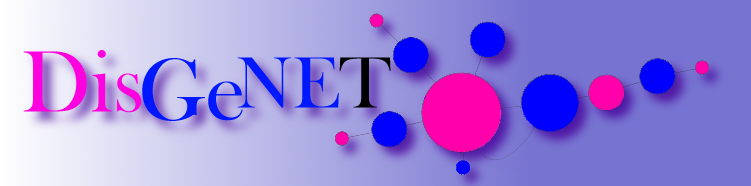
\includegraphics[scale=0.25]{disgenet}
  \vspace*{1 cm}
  \begin{itemize}
    \item Plataforma contendo uma das maiores coleções publicamente disponíveis
          de genes e variantes associados a doenças humanas.
  \end{itemize}
\end{frame}

\begin{frame}
  \frametitle{Outras possibilidades}

  \begin{itemize}
    \item Relacionar Gene-Proteína-Doença (gene codifica proteína que causa doença).
          \begin{itemize}
            \item Permite usar fontes de dados que correlacionam proteínas com doenças.
          \end{itemize}
    \item Interações diretas entre droga e doença (interação de tratamento).
          \begin{itemize}
            \item Poderíamos dizer: droga A previne doença \textalpha, porém
                  aumenta as chances de doença \textgamma.
          \end{itemize}
  \end{itemize}
\end{frame}

\begin{frame}
  \frametitle{Possíveis dificuldades}

  \begin{itemize}
    \item Quantidade muito grande de dados.
          \begin{itemize}
            \item Precisamos coletar dados página por página.
            \item Mais de 10 mil drogas e mais de 100 mil interações no DGIdb.
            \item Coleta pode se tornar lenta.
          \end{itemize}
    \item Confibialidade
          \begin{itemize}
            \item Os dados coletados possuem níveis de confiabilidade
            variáveis, que devem ser levados em conta.
          \end{itemize}
  \end{itemize}
\end{frame}

\begin{frame}[fragile]
  \frametitle{Modelo (protótipo)}

  \begin{alltt}
    Drug(\textcolor{blue}{\underline{DrugId}}, Name, Class)
    DrugAlias(\underline{DrugAlias}, \textcolor{blue}{DrugId})

    Disease(\textcolor{red}{\underline{DiseaseId}}, Name)
    DiseaseAlias(\underline{DiseaseAlias}, \textcolor{red}{DiseaseId})

    Interaction(\textcolor{teal}{\underline{InteractionId}},
                \textcolor{blue}{DrugId},
                \textcolor{red}{DiseaseId},
                InteractionType)
    InteractionSrc(\textcolor{teal}{InteractionId},
                   TrustLevel,
                   Gene,
                   GeneInteractionMechanism,
                   Source)
  \end{alltt}
\end{frame}

\end{document}
